
\subsubsection{Hadronic showers}
High energy hadrons usually interact with matter through nuclear processes, with a much lower cross section than electromagnetic interactions.
\begin{figure}
  \centering 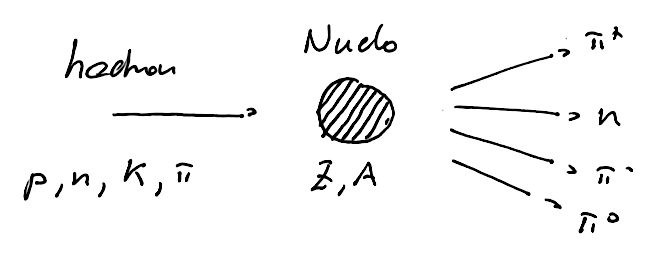
\includegraphics[width=0.4\textwidth]{calo4}
  \caption{}
\item{}
  \label{fig:calo4}
\end{figure}

For hadrons above few $\giga\electronvolt$, the nuclear inelastic cross section does not depend on which hadron is interaction or its energy and it's usually parameterized as:
\[\sigma_{\text{inel}} = \sigma_0 A^{0.7},\qquad \sigma_0 \sim 35\,\milli\barn\]


Elastic interaction are present, but do not contribute to the number of particles and are not considered in the production of hadronic showers, on the other hand, there are many different inelastic process from which many hadrons can be produced, developing hadronic showers.

Nuclear processes which leads to hadronic showers can be classified as:
\begin{itemize}
\item Intra--nuclear showers, in which the nucleus produces hadrons
  \item Inter--nuclear showers, in which secondary particles produced in the collisions interact with other nuclei.
\end{itemize}
The main inelastic process which contribute are:
\begin{itemize}
\item \textbf{Spallation}, in which a collision between two nuclei produces a large number of secondary hadrons. This is the most probable process;
\item \textbf{Nuclear evaporation}, where an excited nucleus undergoes a transition to a stable state releasing hadrons;
  \item \textbf{Nuclear fission}, induced by the capture of slow neutrons from a nucleus (see REF TBA) or after spallation.
\end{itemize}

\begin{figure}
  \centering 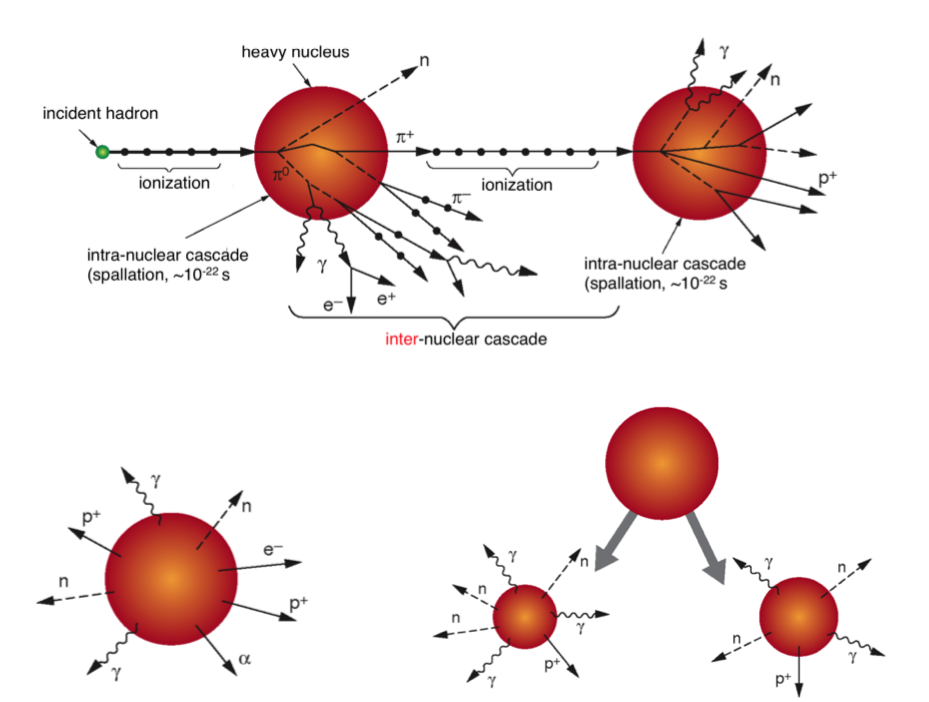
\includegraphics[width=0.9\textwidth]{calo5}
  \caption{Top: Inter--nuclear cascade with spallation. Bottom left: nuclear evaporation. Bottom right: Nuclear fission.}
\item{}
  \label{fig:calo5}
\end{figure}


Among the particles produced in these interaction there are $\pi^0$, which decay immediately in two photons, which starts their electromagnetic shower. Typically the electromagnetic fraction of an hadronic shower (composed of $\gamma$, $e^\pm$, $\pi^0$ and $\eta^0$) is around
\[f_{EM} \sim 30\,\%\]
Also part of the energy is not transferred to the detector material:
\begin{itemize}
\item some nucleus can absorb energy and move to an higher stable state;
\item minimum ionising muons can be produced;
\item neutral stable (or quasi--stable) particles can be produced (neutrinos, $K^0_L$ or neutrons);
\end{itemize}
the detectable part of a shower, via the ionisation of $p$, $\pi$, $K^\pm$, represent $\sim 40\,\%$ of the energy. Since a great fraction of the initial energy can not be detected, hadronic calorimeters have a much lower resolution than e.m. ones.

As analogy to the radiation length $X_0$, it is possible to define the mean hadronic interaction length $\lambda_a$. As shown in section REF TBA, the mean free path for hadronic interaction can be expressed as:
\[\avg{x} = \lambda = \frac{1}{\mu}\]
where $\mu$ is defined as:
\[\mu = \sigma \frac{N_T}{V} = \sigma n_T\]
where $\sigma$ is the inelastic cross section, $N_T$ the number of targets, and $n_T$ the density of targets per unit of volume, which can be written as
\[n_T = \rho\frac{N_A}{A}\]
and finally:
\[\lambda_a = \frac{A}{N_A\rho\sigma}\]
It is immediate to recognise that $\lambda_a$ has the dimension of a length, representing the mean free path crossed by an hadron before undergoing an inelastic nuclear interaction.
\begin{figure}
  \centering 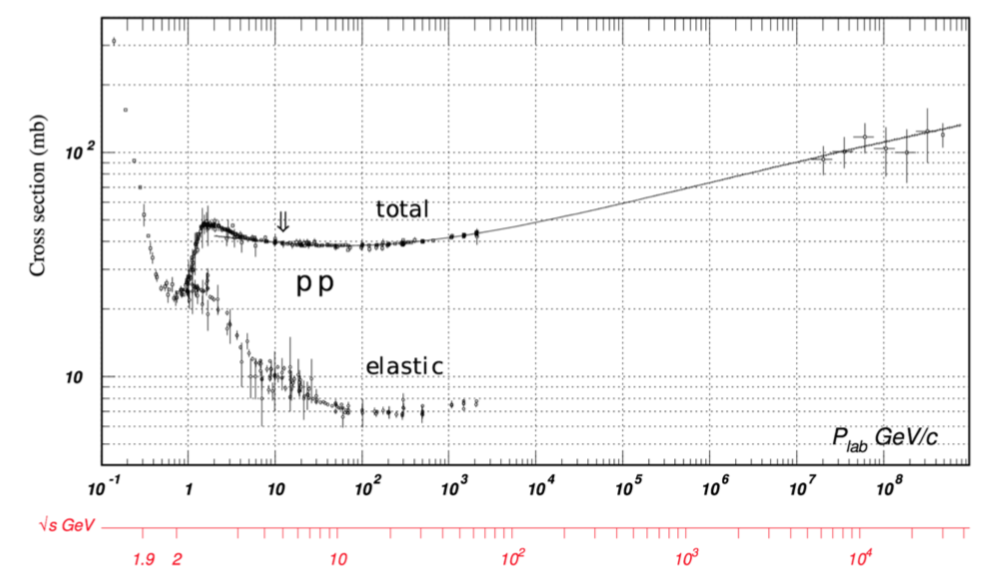
\includegraphics[width=0.9\textwidth]{calo6}
  \caption{Hadronic interaction cross section}
\item{}
  \label{fig:calo6}
\end{figure}

The inelastic hadronic cross section is quite independent on the hadron energy (see figure \ref{fig:calo6}) and grows at high energy.

Hadronic showers can be described in a similar way as electromagnetic showers, let's assume that for each inelastic interaction, which happens after a $\lambda_a$, $\avg{n}$ hadrons are produced. The mean energy of the particles after $t$ steps will be:
\[E_t = \frac{E_0}{\avg{n}^t}\]
and we can consider that under the threshold $E_c\sim 300\,\mega\electronvolt$ hadrons can only interact via elastic scattering or lose their energy by ionisation. This means that the maximum number of particles is given by:
\[E_t = E_c = \frac{E_0}{\avg{n}^t}\]
\[\avg{n}^t = \frac{E_0}{E_c}\]
which gives:
\[t_{\max} = \frac{\ln{\frac{E_0}{E_c}}}{\ln\avg{n}}\]
An approximate formula is the following:
\[t_{\max} = 0.3\ln\rr{E\qq{\giga\electronvolt}}+0.7\]

As shown in figure \ref{fig:calo7}, the development of the shower along the transverse direction is quite larger than the one of electromagnetic showers.
\begin{figure}
  \centering 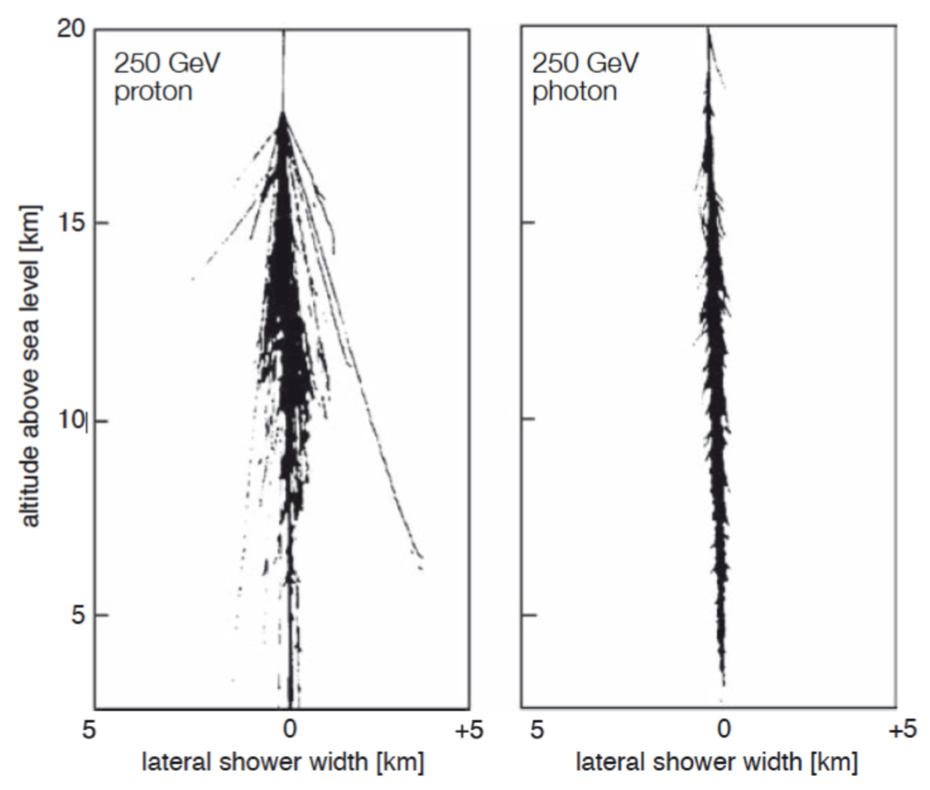
\includegraphics[width=0.9\textwidth]{calo7}
  \caption{}
\item{}
  \label{fig:calo7}
\end{figure}

\begin{figure}
  \centering 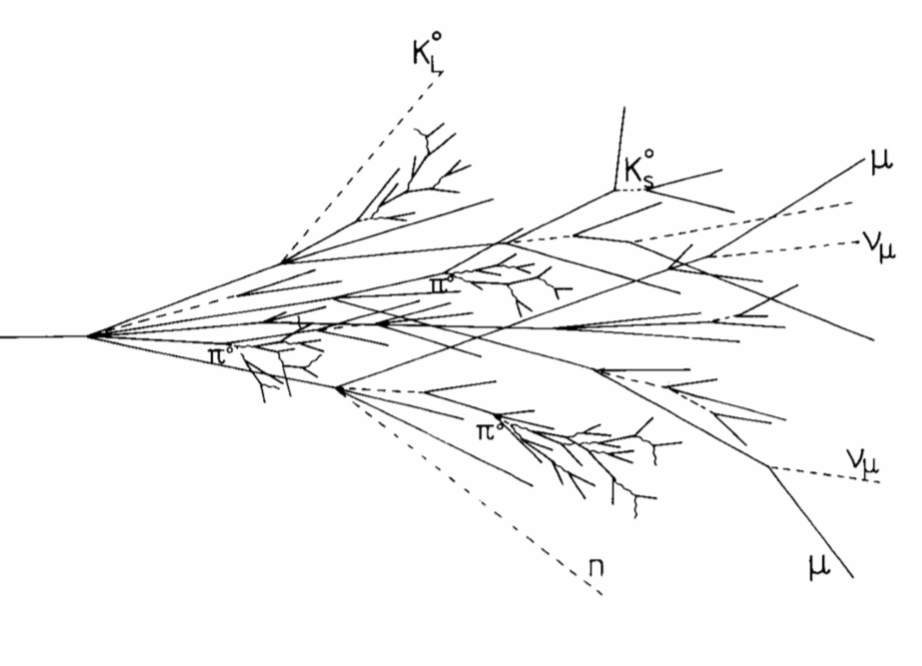
\includegraphics[width=0.5\textwidth]{calo8}
  \caption{}
\item{}
  \label{fig:calo8}
\end{figure}

In a very similar way as electromagnetic calorimeters, many types of different hadronic calorimeters exists, but given also the intrinsic energy loss (which correspond to undetectable energy) there's no necessity to adopt extremely precise solution. Considering also the typical size of an hadronic shower with respect to an e.m. shower (which can be easily imagined looking at the comparison between $\lambda_a$ and $X_0$ in table \ref{tab:detector_lambda_vs_x0}) the size of an hadronic calorimeter needs to be greater, this implies the use of much more material and a greater cost. For these reason hadronic calorimeters are usually based on sampling with high--Z material.
\begin{table}[h!]
  \centering
  \label{tab:detector_lambda_vs_x0}
\begin{tabular}{@{}lll@{}}
\toprule
   & $\lambda_a\,[\centi\meter]$ & $X_0\,[\centi\meter]$ \\ \midrule
Fe & 16.8                        & 1.76                  \\
Pb & 16.9                        & 0.56                  \\
U  & 10.5                        & 0.32                  \\
C  & 98.1                        & 18.8                  \\ \bottomrule
\end{tabular}
\end{table}
Also, by looking at the table \ref{tab:detector_lambda_vs_x0}, it's easy to see how the use of lead is justified for electromagnetic calorimeters, but not necessary for hadronic calorimeters (e.g. ATLAS hadronic calorimeter uses steel as sampling material).

\section{Post Scriptum on Atomic and Nuclear properties and the PDG} 

In addition to providing reviews of the status of all subjects related to particle physics, the Particle Data Group provides a very convenient, clickable page which covers all elements and a number of compounds: \url{https://pdg.lbl.gov/2020/AtomicNuclearProperties/index.html}. All properties that have been discussed in this chapter are available, such as atomic and mass numbers, mean ionization (excitation) energies, minimum of ionization, as well as $dE/dx$ and range tables. 


\section*{Take-home lessons}
\begin{itemize}
    \item When an incoming particle travels in a medium with a refraction index $n$, and its speed is higher than the speed of light in the medium ($c/n$), the atoms along the particle path will be polarised and release radiation in spherical waves. These waves interfere constructively, with the result that one observes an envelope (\emph{Cerenkov radiation}) at an angle $\theta_c = \arccos{1/\beta n}$. From classical electrodynamics, the number of emitted photons per unit path length of the incoming particle depends on the charge of the incoming particle and $\theta_c$, $\langle \od{n}{x}\approx \SI{600}{photons/cm} z^2 \sin^2\theta_c$. Cerenkov emission does not contribute significantly to the energy loss of a particle, as its intensity is much lower than ionisation energy loss ($\approx\SI{2}{keV}$, to be compared to \od{E}{x} from the Bethe-Bloch formula).
    \item When a charged particle is decelerated by an electric field, it emits \emph{bremsstrahlung} radiation. The energy released per unit path length of the incoming particle is usually expressed in the form $\od{E}{X}\approx E/X_0$, where $X_0$ is the \emph{radiation length} and depends on the medium. 
    \item The \emph{critical energy} of a particle is the energy at which the ionisation and radiation energy loss are equal. This quantity depends on the atomic number of the material and on the kind of particle.
    \item Incoming particles can also interact with the Coulomb field of atomic nuclei, in an extension of Rutherford scattering to multiple collisions. Since the Rutherford cross-section depends on the scattering angle as $\sin^{-4}\theta/2$, the most probable angle will be $\langle\theta\rangle=0$, and one can assume a Gaussian distribution of $\theta$ centered at zero. The variance of this Gaussian can be calculated (again, after having expressed the minimum and maximum values of $\theta$ as a function of the minimum and maximum impact parameter values), and depends on the particle charge, the inverse of its velocity and the square root of its path length, normalised to $X_0$.
    \item Photons which travel a material with an energy between the ionisation energy of the material and $\approx\SI{100}{keV}$ dominantly interact with matter through the \emph{photoelectric effect}. The photon interacts with the atomic electron (as required by the conservation of four-momentum!) and extracts the electron from the atom. The cross-section of this process depends on the atomic number of the material, $Z$, and on the energy of the photon, $\sigma \propto Z^5/E^3$. Experimentally, one can observe "spikes" in the measured cross-section in correspondence of the various atomic electron shells.
    \item Photons with higher energy effectively see the atomic electrons as unbound, and undergo Compton scattering. The energy of the scattered photon depends on the scattering angle via simple relativistic kinematics. The maximum released energy corresponds to the minimum photon energy and is called \emph{Compton edge}: experimentally, it is the point at which the spectrum of the energy released to the material has a cutoff.
    \item Photons can also undergo two purely classical processes, Thomson scattering and Rayleigh scattering. Thomson scattering happens when photons have less energy than the electron mass, and electrons can be considered as free: the electron oscillates under the presence of the photon electromagnetic wave, and emits a secondary spherical wave. Rayleigh scattering happens when the whole atom takes part to the elastic scattering with the photon (\emph{coherent scattering}). These two processes are practically negligible for photons with sufficiently high energy.
    \item Photons with sufficiently high energy can produce, in the presence of a nucleus or of an electron (again, as required by the conservation of four-momentum!), an electron-positron pair. The kinematic threshold for the process in presence of the nucleus (electrons) is $2m_e$ ($4m_e$).  The cross-section of this process for sufficiently high-energy photons grows linearly with the atomic number of the material (or, equivalently, with the ratio between its atomic mass number and $X_0$).
    \item Electrons and positrons above their critical energy, or photons above the pair-production threshold, can start a cascade process which leads to the production of many of these particles in the material. This process is called \emph{electromagnetic shower} and its longitudinal and lateral development can be expressed as a function of the ratio between the energy of the particle which started the shower and the electron critical energy in the material.
\end{itemize}
\section*{Questions}
\begin{itemize}
    \item Do neutrons produce Cerenkov radiation?
\end{itemize}


%%%Local Variables:
%%% mode: latex
%%% TeX-master: "../book"
%%% End:
